\ifx\wholebook\relax \else
% ------------------------

\documentclass[UTF8]{article}
%------------------- Other types of document example ------------------------
%
%\documentclass[twocolumn]{IEEEtran-new}
%\documentclass[12pt,twoside,draft]{IEEEtran}
%\documentstyle[9pt,twocolumn,technote,twoside]{IEEEtran}
%
%-----------------------------------------------------------------------------
%
% loading packages
%

\RequirePackage{ifpdf}
\RequirePackage{ifxetex}

%
%
\ifpdf
  \RequirePackage[pdftex,%
       bookmarksnumbered,%
              colorlinks,%
          linkcolor=blue,%
              hyperindex,%
        plainpages=false,%
       pdfstartview=FitH]{hyperref}
\else\ifxetex
  \RequirePackage[bookmarksnumbered,%
               colorlinks,%
           linkcolor=blue,%
               hyperindex,%
         plainpages=false,%
        pdfstartview=FitH]{hyperref}
\else
  \RequirePackage[dvipdfm,%
        bookmarksnumbered,%
               colorlinks,%
           linkcolor=blue,%
               hyperindex,%
         plainpages=false,%
        pdfstartview=FitH]{hyperref}
\fi\fi
%\usepackage{hyperref}

% other packages
%--------------------------------------------------------------------------
\usepackage{graphicx, color}
\usepackage{subfig}
\usepackage{tikz}
\usetikzlibrary{matrix,positioning}

\usepackage{amsmath, amsthm, amssymb} % for math
\usepackage{exercise} % for exercise
\usepackage{import} % for nested input

%
% for programming
%
\usepackage{verbatim}
\usepackage{listings}
%\usepackage{algorithmic} %old version; we can use algorithmicx instead
\usepackage{algorithm}
\usepackage[noend]{algpseudocode} %for pseudo code, include algorithmicsx automatically
\usepackage{appendix}
\usepackage{makeidx} % for index support
\usepackage{titlesec}

\usepackage[cm-default]{fontspec}
\usepackage{xunicode}

% detect and select Chinese font
% ------------------------------
% the following cmd can list all availabe Chinese fonts in host.
% fc-list :lang=zh
\def\myfont{STHeiti}  % Under Mac OS X
\def\linuxfallback{WenQuanYi Micro Hei} % Under Linux
\def\winfallback{SimSun} % Under Windows
\suppressfontnotfounderror1 % Avoid setting exit code (error level) to break make process
\count255=\interactionmode
\batchmode
\font\foo="\myfont"\space at 10pt
\ifx\foo\nullfont
  \font\foo = "\linuxfallback"\space at 10pt
  \ifx\foo\nullfont
    \font\foo = "\winfallback"\space at 10pt
    \ifx\foo\nullfont
      \errorstopmode
      \errmessage{no suitable Chinese font found}
    \else
      \let\myfont=\winfallback % Windows
    \fi
  \else
    \let\myfont=\linuxfallback % Linux
  \fi
\fi
\interactionmode=\count255
\setmainfont[Mapping=tex-text]{\myfont}

\XeTeXlinebreaklocale "zh"  % to solve the line breaking issue
\XeTeXlinebreakskip = 0pt plus 1pt minus 0.1pt

\titleformat{\paragraph}
{\normalfont\normalsize\bfseries}{\theparagraph}{1em}{}
\titlespacing*{\paragraph}
{0pt}{3.25ex plus 1ex minus .2ex}{1.5ex plus .2ex}

\lstdefinelanguage{Smalltalk}{
  morekeywords={self,super,true,false,nil,thisContext}, % This is overkill
  morestring=[d]',
  morecomment=[s]{"}{"},
  alsoletter={\#:},
  escapechar={!},
  literate=
    {BANG}{!}1
    {UNDERSCORE}{\_}1
    {\\st}{Smalltalk}9 % convenience -- in case \st occurs in code
    % {'}{{\textquotesingle}}1 % replaced by upquote=true in \lstset
    {_}{{$\leftarrow$}}1
    {>>>}{{\sep}}1
    {^}{{$\uparrow$}}1
    {~}{{$\sim$}}1
    {-}{{\sf -\hspace{-0.13em}-}}1  % the goal is to make - the same width as +
    %{+}{\raisebox{0.08ex}{+}}1		% and to raise + off the baseline to match -
    {-->}{{\quad$\longrightarrow$\quad}}3
	, % Don't forget the comma at the end!
  tabsize=2
}[keywords,comments,strings]

% for better Haskell code outlook
\lstdefinelanguage{Haskell}{
  basicstyle=\small\ttfamily,
  flexiblecolumns=false,
  basewidth={0.5em,0.45em},
  literate={+}{{$+$}}1 {/}{{$/$}}1 {*}{{$*$}}1 {=}{{$=$}}1
           {>}{{$>$}}1 {<}{{$<$}}1 {\\}{{$\lambda$}}1
           {\\\\}{{\char`\\\char`\\}}1
           {->}{{$\rightarrow$}}2 {>=}{{$\geq$}}2 {<-}{{$\leftarrow$}}2
           {<=}{{$\leq$}}2 {=>}{{$\Rightarrow$}}2
           {\ .}{{$\circ$}}2 {\ .\ }{{$\circ$}}2
           {>>}{{>>}}2 {>>=}{{>>=}}2
           {|}{{$\mid$}}1
}[keywords,comments,strings]

\lstloadlanguages{C, C++, Lisp, Haskell, Python, Smalltalk}

\lstset{
  showstringspaces = false
}

% ======================================================================

\def\BibTeX{{\rm B\kern-.05em{\sc i\kern-.025em b}\kern-.08em
    T\kern-.1667em\lower.7ex\hbox{E}\kern-.125emX}}

%
% mathematics
%
\newcommand{\be}{\begin{equation}}
\newcommand{\ee}{\end{equation}}
\newcommand{\bmat}[1]{\left( \begin{array}{#1} }
\newcommand{\emat}{\end{array} \right) }
\newcommand{\VEC}[1]{\mbox{\boldmath $#1$}}

% numbered equation array
\newcommand{\bea}{\begin{eqnarray}}
\newcommand{\eea}{\end{eqnarray}}

% equation array not numbered
\newcommand{\bean}{\begin{eqnarray*}}
\newcommand{\eean}{\end{eqnarray*}}

\newtheorem{theorem}{Theorem}[section]
\newtheorem{lemma}[theorem]{Lemma}
\newtheorem{proposition}[theorem]{Proposition}
\newtheorem{corollary}[theorem]{Corollary}


\setcounter{page}{1}

\begin{document}

%--------------------------

% ================================================================
%                 COVER PAGE
% ================================================================

\title{后缀树}

\author{刘新宇
\thanks{{\bfseries 刘新宇 } \newline
  Email: liuxinyu95@gmail.com \newline}
  }

\maketitle
\fi

\markboth{后缀树}{初等算法}

\ifx\wholebook\relax
\chapter{后缀树}
\numberwithin{Exercise}{chapter}
\fi

%{\bfseries Corresponding Author:} Larry LIU Xinyu

% ================================================================
%                 Introduction
% ================================================================
\section{简介}
\label{introduction}
\index{后缀树}

后缀树是一种重要的数据结构,它可以用来实现很多快速的字符串操作算法\cite{wiki-suffix-tree}。后缀树还在生物信息处理中被广泛应用于DNA模式匹配\cite{ukkonen-presentation}。Weiner在1973年最早介绍了后缀树\cite{weiner73},最新的on-line构造算法发现于1995年\cite{ukkonen95}。

字符串$S$的后缀树是一棵特殊的Patricia(见上一章Radix树的介绍)。树中的所有边都由$S$的某个子串标记。$S$的每个后缀都唯一对应一条从根到叶子的路径。图\ref{fig:stree-banana}显示了一棵对应英文单词‘banana’的后缀树。

\begin{figure}[htbp]
  \centering
  \includegraphics[scale=0.5]{img/stree-banana.ps}
  \caption{英文“banana”对应的后缀树。} \label{fig:stree-banana}
\end{figure}

所有的后缀“banana”、“anana”、“nana”、“ana”、“na”、
“a”和空串“”都可以在上面的后缀树中找到。这些后缀中,前三个存在明确的对应路径,其余的并未明确显示出来。这是因为后面四个后缀:“ana”、
“na”、“a”和空串“”同时也是其他后缀的前缀。为了将所有后缀都明确显示出来,我们可以在原字符串的末尾附加一个特殊的终结符,这一终结符不在字符串的其他位置出现过。我们通常把它标记为‘\$’。这样,就不存在任何后缀同时也是其他某个后缀的前缀。

虽然字符串“banana”的后缀树很简单,但是字符串“bananas”的后缀树却大相径庭。如图\ref{fig:stree-bananas}所示。

\begin{figure}[htbp]
  \centering
  \includegraphics[scale=0.5]{img/stree-bananas.ps}
  \caption{字符串“bananas”对应的后缀树} \label{fig:stree-bananas}
\end{figure}

我们可以复用上一章中介绍过的Patricia插入算法来构造后缀树。

\begin{algorithmic}[1]
\Function{Suffix-Tree}{$S$}
  \State $T \gets$ NIL
  \For{$i \gets 1$ to $|S|$}
    \State $T \gets$ \textproc{Patricia-Insert}($T$, \Call{Right}{$S, i$})
  \EndFor
  \State \Return $T$
\EndFunction
\end{algorithmic}

对于非空字符串$S=s_1s_2...s_i...s_n$,长度$n = |S|$,函数\textproc{Right}($S, i$) $= s_is_{i+1...s_n}$。它的结果是一个子串,从$S$的第$i$个字符直到末尾。这一直观的算法也可以定义如下:

\be
suffix_T(S) = fold(insert_{Patricia}, \phi, suffixes(S))
\ee

其中函数$suffixes(S)$枚举字符串$S$的所有后缀。如果字符串为空,结果是一个空串;否则$S$本身是自己的一个后缀,其余后缀可以通过递归调用$suffixes(S')$来获取。这里$S'$是$S$除去第一个字符以外的其他字符。

\be
suffixes(S) = \left \{
  \begin{array}
  {r@{\quad:\quad}l}
  \{ \phi \} & S = \phi \\
  \{S\} \cup suffixes(S') & otherwise
  \end{array}
\right.
\ee

对于长度为$n$的字符串,这一方法需要$O(n^2)$的时间来构造后缀树。这是因为它总共将$n$个后缀插入到树中,而每次插入的时间和后缀的长度成正比。算法的性能不够好。

本章中,我们首先介绍一种快速的on-line后缀trie的构造方法,它使用了后缀链接(suffix link)的概念。由于trie耗费大量的空间,我们接下来介绍一种由Ukkonen发现的线性时间的on-line后缀树构造算法。最后,我们介绍如何使用后缀树来解决一些字符串处理的有趣问题。

% ================================================================
%                 Suffix Trie
% ================================================================
\section{后缀trie}
\label{suffix-trie}
\index{后缀trie}

如同trie和Patricia的关系,后缀trie比后缀树的结构简单许多。图\ref{fig:strie-banana}是英文单词“banana”对应的后缀trie。

\begin{figure}[htbp]
  \centering
  \includegraphics[scale=0.4]{img/strie-banana.ps}
  \caption{“banana”对应的后缀trie。} \label{fig:strie-banana}
\end{figure}

和图\ref{fig:stree-banana}比较,我们可以发现后缀树和后缀trie的区别。后缀trie中的每条边仅仅代表一个字符,而不是一个子串。因此后缀trie需要使用更多的空间来存储信息。如果我们将只含有一个子树的节点压缩到一起,后缀trie就转变成一棵后缀树。

我们可以复用trie的定义:每个节点对应一个字符,节点包含多个子树。子树可以通过对应的字符来引用。

% ================================================================
%               Online construction of Suffix Trie
% ================================================================
\subsection{节点转移和后缀链接}

设字符串$S$的长度为$n$,定义$S_i=s_1s_2...s_i$为包含前$i$个字符的前缀。

\index{后缀树!节点转移}
在后缀trie中,每个节点都代表一个后缀。如图\ref{fig:strie-cacao}所示的例子,节点$X$代表后缀“a”,通过添加字符‘c’,节点$X$转移到节点$Y$,节点$Y$代表后缀“ac”。我们称节点$X$通过代表字符‘c’的边转移到节点$Y$\cite{ukkonen95}。

\begin{figure}[htbp]
  \centering
  \includegraphics[scale=0.45]{img/strie-cacao.ps}
  \caption{字符串‘cacao’对应的后缀trie。节点$X \gets$ “a”、节点$Y \gets$ “ac”,节点$X$通过字符‘c’转移到$Y$。}
  \label{fig:strie-cacao}
\end{figure}

\begin{algorithmic}
\State $Y \gets$ \Call{Children}{$X$}[$c$]
\end{algorithmic}

同时,我们也称节点$X$有一个‘c’子节点$Y$。下面的Python表达式给出了一个节点转移的一个例子。

\lstset{language=python}
\begin{lstlisting}
y = x.children[c]
\end{lstlisting}

\index{后缀链接}
如果后缀trie中的节点$A$代表后缀$s_is_{i+1}...s_n$,节点$B$代表后缀$s_{i+1}s_{i+2}...s_n$,我们称节点$B$代表节点$A$的\underline{后缀}。我们可以创建一个从$A$到$B$的链接,称为节点$A$的\underline{后缀链接}\cite{ukkonen95}。我们通常用虚线箭头来表示后缀链接。在图\ref{fig:strie-cacao}的例子中,节点$A$的后缀链接指向节点$B$,节点$B$的后缀链接指向节点$C$。

除根节点外,所有的节点都存在后缀链接。为此我们在trie的定义中增加一个后缀链接的部分,如下面的Python例子代码所示。

\lstset{language=Python}
\begin{lstlisting}
class STrie:
    def __init__(self, suffix=None):
        self.children = {}
        self.suffix = suffix
\end{lstlisting}

\subsection{On-line构造}
\index{后缀trie!on-line构造}

对于字符串$S$,假设我们已经构造了第$i$个前缀$S_i=s_1s_2...s_i$的后缀trie。记这一后缀trie为$SuffixTrie(S_i)$。我们考虑如何从$SuffixTrie(S_i)$获得$SuffixTrie(S_{i+1})$。

如果列出$SuffixTrie(S_i)$中的全部后缀,按照从最长的(就是$S_i$本身)到最短的(为空串)的顺序,我们可以获得表\ref{tab:suffixes_s_i}。总共有$i+1$个后缀。

\begin{table}
  \begin{tabular}{r}
    后缀 \\
    $s_1s_2s_3...s_i$ \\
    $s_2s_3...s_i$ \\
    ... \\
    $s_{i-1}s_i$ \\
    $s_i$ \\
    “” \\
  \end{tabular}
  \caption{$S_i$的全部后缀}
  \label{tab:suffixes_s_i}
\end{table}

我们可以向表中的每个后缀后面添加字符$s_{i+1}$,然后再增加一个空串。这样就获得了$S_{i+1}$的全部后缀。这等效于给trie中的所有节点增加一个代表字符$s_{i+1}$的新节点。

\begin{algorithm}
\begin{algorithmic}[1]
\For{$\forall T \in SuffixTrie(S_i)$}
  \State \Call{Children}{$T$}[$s_{i+1}$] $\gets$ \Call{Create-Empty-Node}{}
\EndFor
\end{algorithmic}
\caption{从$SuffixTrie(S_i)$获取$SuffixTrie(S_{i+1})$,最初的版本。}
\label{algo:strie1}
\end{algorithm}

但是,$SuffixTrie(S_i)$中的某些节点可能已经有$s_{i+1}$子节点了。例如,图\ref{fig:strie-cac}中,节点$X$和节点$Y$分别代表后缀“cac”和“ac”。它们没有‘a’子节点;但是代表后缀“c”的节点$Z$,已经有‘a’子节点了。

\begin{figure}[htbp]
  \centering
  \subfloat[字符串“cac”对应的后缀trie。]{\hspace{.2\textwidth}\includegraphics[scale=0.5]{img/strie-cac.ps}\hspace{.2\textwidth}}
  \subfloat[字符串“caca”对应的后缀trie。]{\hspace{.2\textwidth}\includegraphics[scale=0.5]{img/strie-caca.ps}\hspace{.2\textwidth}}
  \caption{字符串“cac”和“caca”对应的后缀trie。}
  \label{fig:strie-cac}
\end{figure}

当向$SuffixTrie(S_i)$增加字符$s_{i+1}$(这里$s_{i+1}$为‘a’)时,我们需要为$X$和$Y$新建子节点,但是我们不需要给$Z$新建子节点。

如果我们逐一检查表\ref{tab:suffixes_s_i}中的每一项,当发现一个节点已经有$s_{i+1}$子节点时,我们可以立即停止。这是因为,如果$SuffixTrie(S_i)$中的节点$X$已经有$s_{i+1}$子节点,根据后缀连接的定义,$SuffixTrie(S_i)$中任何$X$的后缀节点$X'$一定也存在$s_{i+1}$子节点。也就是说,设$c=s_{i+1}$,若$wc$是$S_i$的子串,则$wc$的每个前缀也都是$S_i$的子串\cite{ukkonen95}。唯一的例外是根节点,因为根节点代表空串“”。

根据上面的分析,我们可以将算法\ref{algo:strie1}改进如下:

\begin{algorithm}
  \begin{algorithmic}[1]
  \For{each $T \in SuffixTrie(S_i)$ in descending order of suffix length}
    \If{\Call{Children}{$T$}[$s_{i+1}$] = NIL}
      \State \Call{Children}{$T$}[$s_{i+1}$] $\gets$ \Call{Create-Empty-Node}{}
    \Else
      \State break
    \EndIf
  \EndFor
  \end{algorithmic}
  \caption{从$SuffixTrie(S_i)$获取$SuffixTrie(S_{i+1})$,改进版本}
  \label{algo:strie2}
\end{algorithm}

接下来的问题是如何按照后缀的长度,从长到短降序遍历所有的节点?我们定义一棵后缀trie的\underline{top}为深度最大的叶子节点。这一定义保证了top指向最长的后缀。我们从top开始,沿着后缀连接每前进一步,后缀的长度就相应减一。沿着后缀连接我们可以一直从top遍历到root。这一遍历的顺序恰好符合我们的要求。最后,我们需要处理一棵特殊的trie―$SuffixTrie(NIL)$,它对应空串。这种情况下,我们定义top和root相等。

\begin{algorithmic}
\Function{Insert}{$top, c$}
  \If{$top = $ NIL} \Comment{The trie is empty}
    \State $top \gets$ \Call{Create-Empty-Node}{}
  \EndIf
  \State $T \gets top$
  \State $T' \gets$ \Call{Create-Empty-Node}{} \Comment{dummy init value}
  \While{$T \neq$ NIL $\land$ \Call{Children}{$T$}[$c$] = NIL}
    \State \Call{Children}{$T$}[$c$] $\gets$ \Call{Create-Empty-Node}{}
    \State \Call{Suffix-Link}{$T'$} $\gets$ \Call{Children}{$T$}[$c$]
    \State $T' \gets$ \Call{Children}{$T$}[$c$]
    \State $T \gets$ \Call{Suffix-Link}{$T$}
  \EndWhile
  \If{$T \neq$ NIL}
    \State \Call{Suffix-Link}{$T'$} $\gets$ \Call{Children}{$T$}[$c$]
  \EndIf
  \State \Return \Call{Children}{$top$}[$c$] \Comment{returns the new top}
\EndFunction
\end{algorithmic}

函数\textproc{Insert}从$SuffixTrie(S_i)$构造$SuffixTrie(S_{i+1})$。它接受两个参数:一个是$SuffixTrie(S_i)$的top位置,另外一个是字符$s_{i+1}$。如果top为空(NIL),说明树也是空的,根节点root也就不存在。这种情况下我们需要创建一个root。我们使用一个空节点$T'$作为sentinel。它可以用来记录上一次创建的新节点。在主循环中,算法沿着后缀连接逐一检查每个节点。如果$s_{i+1}$子节点不存在,就创建一个新节点,并将其对应到字符$s_{i+1}$上。算法不断沿着后缀连接遍历直到根节点root,或者中途遇到一个已经有$s_{i+1}$子节点的位置。这时,最后一个后缀连接指向这一子节点。最后算法返回新的top位置用于将后继字符插入到后缀trie中。

给定字符串$S$,我们可以通过不断调用\textproc{Insert}函数来构造后缀trie。

\begin{algorithmic}[1]
\Function{Suffix-Trie}{$S$}
  \State $t \gets$ NIL
  \For{$i \gets 1$ to $|S|$}
    \State $t \gets$ \Call{Insert}{$t, s_i$}
  \EndFor
  \State \Return $t$
\EndFunction
\end{algorithmic}

注意:这一算法的返回值不是根节点,而是后缀trie的top节点。我们可以通过沿着后缀连接遍历以获得根节点。

\begin{algorithmic}[1]
\Function{Root}{$T$}
  \While{\Call{Suffix-Link}{$T$} $\neq$ NIL}
    \State $T \gets$ \Call{Suffix-Link}{$T$}
  \EndWhile
  \State \Return $T$
\EndFunction
\end{algorithmic}

图\ref{fig:cons-strie-cacao}给出了构造字符串“cacao”后缀树的步骤。简单起见,我们只画出了最后的一组后缀连接。

\begin{figure}[htbp]
  \centering
  \subfloat[空]{\hspace{.1\textwidth}\includegraphics[scale=0.5]{img/strie-empty.ps}\hspace{.1\textwidth}}
  \subfloat[“c”]{\hspace{.1\textwidth}\includegraphics[scale=0.5]{img/strie-c.ps}\hspace{.1\textwidth}}
  \subfloat[“ca”]{\hspace{.1\textwidth}\includegraphics[scale=0.5]{img/strie-ca.ps}\hspace{.1\textwidth}} \\
  \subfloat[“cac”]{\hspace{.1\textwidth}\includegraphics[scale=0.5]{img/strie-cac.ps}\hspace{.1\textwidth}}
  \subfloat[“caca”]{\hspace{.1\textwidth}\includegraphics[scale=0.5]{img/strie-caca.ps}\hspace{.1\textwidth}}
  \subfloat[“cacao”]{\hspace{.1\textwidth}\includegraphics[scale=0.5]{img/strie-cacao.ps}\hspace{.1\textwidth}}
  \caption{构造字符串“cacao”的后缀trie。共分6步。虚线箭头表示最后一组后缀连接。}
  \label{fig:cons-strie-cacao}
\end{figure}

由于每次沿着后缀连接遍历,算法\textproc{Insert}的时间复杂度和后缀trie的大小成正比。最坏情况下,对于长度为$n$的字符串,需要$O(n^2)$时间来构造后缀trie。例如字符串$S=a^nb^n$,有$n$个字符$a$和$n$个字符$b$,就可使得算法的性能严重下降。

下面的Python例子程序实现了后缀trie的构造算法。

\lstset{language=Python}
\begin{lstlisting}
def suffix_trie(str):
    t = None
    for c in str:
        t = insert(t, c)
    return root(t)

def insert(top, c):
    if top is None:
        top=STrie()
    node = top
    new_node = STrie() #dummy init value
    while (node is not None) and (c not in node.children):
        new_node.suffix = node.children[c] = STrie(node)
        new_node = node.children[c]
        node = node.suffix
    if node is not None:
        new_node.suffix = node.children[c]
    return top.children[c] #update top

def root(node):
    while node.suffix is not None:
        node = node.suffix
    return node
\end{lstlisting}

% ================================================================
%               Suffix Tree
% ================================================================
\section{后缀树}
\index{后缀树}

后缀trie既耗费空间,构造起来又慢(平方时间复杂度)。有些实现仅仅将构后缀trie压缩成后缀树\cite{trivial-stree-java},但是这样还不够理想。Ukkonen在1995年发表了一种高效的on-line构造算法,可以达在线性时间内构造后缀树。

% ================================================================
%               Online construction of suffix tree
% ================================================================
\subsection{on-line构造}

\subsubsection{Active point和end point}
\label{ap-and-ep}
\index{后缀树!active point}
\index{后缀树!end point}

在后缀trie构造算法中,我们可以从任意一个中间结果$SuffixTrie(S_i)$得到下一个结果$SuffixTrie(S_{i+1})$。这一点很具有启发性。我们观察一下图\ref{fig:cons-strie-cacao}中的最后两步。

一共有两种不同的更新:
\begin{enumerate}
\item 所有的叶子节点都添加了一个代表字符$s_{i+1}$的新节点;
\item 某些中间节点被分支出一个代表字符$s_{i+1}$的新节点。
\end{enumerate}

其中第一种更新很简单易懂,我们总是要为下一个字符增加新节点。Ukkonen将所有的叶子节点定义为“开放节点”。

我们更加关心第二种更新。什么样的中间节点会被分支出新节点?我们希望能快速定位到它们,以实施更新。

Ukkonen将从top沿着后缀连接前进的路径定义为“boundary路径”。记boundary路径上的各个节点为$n_1, n_2, ..., n_j, ..., n_k$。显然,第一个是叶子节点(为top),假设从第$j$个节点开始不再是叶子节点,此后我们需要不断分支出新节点直到处理完第$k$个。

Ukkonen将此路径上的第一个非叶子节点$n_j$定义为“active point”,最后一个节点$n_k$定义为“end point”,它有可能是根节点root。

\subsubsection{引用对(Reference pair)}
\index{后缀树!reference pair}

\begin{figure}[htbp]
  \centering
  \includegraphics[scale=0.5]{img/stree-bananas-label.ps}
  \caption{字符串“bananas”的后缀树。节点$X$通过子串“na”转移到节点$Y$。}
  \label{fig:stree-bananas-label}
\end{figure}

图\ref{fig:stree-bananas-label}是字符串“bananas”对应的后缀树。节点$X$代表后缀“a”。通过添加子串“na”,节点$X$转移到代表后缀“ana”的节点$Y$。也就是说,我们可以将$Y$表达为一对值,由一个节点和一个子串组成。形如$(X, w)$,其中$w=$“na”。

Ukkonen称这样的一对值为\underline{引用对}(reference pair)。不光所有的可见节点,而且连不可见的隐藏节点都可以用引用对来表示。例如$(X$, “n” $)$就表达了图\ref{fig:stree-bananas-label}中一个隐藏节点的位置。通过使用引用对,我们可以定位到后缀树中的任何位置。

给定字符串$S$,它的所有子串都可以用一对索引$(l, r)$来确定。其中,$l$是子串最左侧字符的索引,而$r$是最右侧字符的索引。例如,若字符串$S=$“bananas”,并且索引从1开始,子串“na”可以表达为一对索引$(3, 4)$。通过使用索引对,我们可以仅仅保留一份字符串的完整拷贝,从而大量节省空间。后缀树中的任何位置都可以定义为形如$(node, (l, r))$的表达式。这就是引用对的最终形式。

利用引用对,后缀树中的节点转移可以定义如下:

\textproc{Children}($X$)[$s_l$] $\gets ((l, r), Y) \iff Y \gets (X, (l, r))$

若字符$s_l=c$,我们称节点$X$有一个$c$子节点$Y$。$Y$可以由$X$通过子串$(l, r)$转移到。每个节点最多有一个$c$子节点。

\subsubsection{归一化引用对}
\index{后缀树!归一化引用对}

显然,后缀树中的一个位置可能存在多个引用对。例如图\ref{fig:stree-bananas-label}中的节点$Y$既可以表示为引用对$(X, (3, 4))$,也可以表示为$(root, (2, 4))$。如果我们定义空串为$\epsilon=(i, i-1)$,$Y$还可以表示为$(Y, \epsilon)$。

所谓归一化引用对,是指含有距离一个位置最近的节点的引用对。特别地,对于后缀树中的某个节点,归一化引用对含由该节点和空串组成。所以节点$Y$的归一化引用对为$(Y, \epsilon)$。

下面的算法将任一引用对$(node, (l, r))$转换为归一化引用对$(node', (l', r))$。由于转换后$r$不会变,所以算法仅仅返回$(node', l')$作为结果。

\begin{algorithm}
\begin{algorithmic}[1]
\Function{Canonize}{$node, (l, r)$}
  \If{$node = $ NIL}
    \If{$(l, r) = \epsilon$}
      \State \Return $($ NIL, $l)$
    \Else
      \State \Return \Call{Canonize}{$root, (l+1, r)$}
    \EndIf
  \EndIf
  \While{$l \leq r$} \Comment{$(l, r) isn't empty $}
    \State $((l', r'), node') \gets$ \Call{Children}{$node$}[$s_l$]
    \If{$ r-l \geq r'-l'$}
      \State $l \gets l + r' - l' + 1$ \Comment{Remove $|(l', r')|$ chars from $(l, r)$}
      \State $node \gets node'$
    \Else
      \State break
    \EndIf
  \EndWhile
  \State \Return $(node, l)$
\EndFunction
\end{algorithmic}
\caption{将任一引用对转换为归一化引用对}
\label{algo:canon}
\end{algorithm}

算法需要单独处理传入空节点NIL的情况。此时算法必定按照下面的方式调用:

\textproc{Canonize}(\textproc{Suffix-Link}($root$), $(l, r)$)

由于根节点的后缀连接为空NIL,若子串$(l, r)$不等于$\epsilon$,则结果为$(root, (l+1, r))$;否则,我们应该返回一个特殊的结束位置:$($NIL, $\epsilon)$。

我们将稍后详细解释这一特殊情况。

\subsubsection{Ukkonen算法}
\index{后缀树!on-line构造}
\index{Ukkonen算法}

我们在前面\ref{ap-and-ep}一节中提到,为所有的叶子添加代表新字符的节点很简单。使用引用对的概念,当我们从后缀树$SuffixTree(S_i)$更新到$SuffixTree(S_{i+1})$时,所有形如$(node, (l, i))$的节点都是叶子节点。它们将更新为$(node, (l, i+1))$。Ukkonen为此将叶子表示为$(node, (l, \infty))$,其中无穷$\infty$的含义是“增长开放”
(open to grow)。在后缀树构造过程中,我们可以暂时忽略全部的叶子节点。当构造完毕后,只要把引用对中的无穷$\infty$替换为字符串的长度就可以了。

这样,算法仅仅关注从active point到end point这条路径上的所有\underline{位置}。最关键的问题是如何找到active point和end ponit。

当开始构造后缀树时,仅仅存在一个根节点。没有任何分支和叶子。因此active point为$(root, \epsilon)$,或者表示为$(root, (1, 0))$(字符串从1开始索引)。

而end point,它是更新$SuffixTree(S_i)$过程停止时的未知。根据后缀trie算法,我们知道在它的\underline{位置}上,已经存在$s_{i+1}$子节点了。注意:后缀trie中的某个节点不一定是后缀树中的可见节点。若$(node, (l, r))$是end point,则可能存在两种情况:

\begin{enumerate}
\item $(l, r)=\epsilon$。这说明end point是一个可见节点。该节点含有一个$s_{i+1}$子节点,亦即\textproc{Children}($node$)[$s_{i+1}$] $\neq$ NIL;
\item 否则,$l \leq r$,说明end point是一个隐藏的位置。我们有$s_{i+1}=s_{l'+|(l, r)|}$,
\textproc{Children}($node$)[$s_l$]$=((l', r'), node')$,这里$|(l, r)|$表示子串$(l, r)$的长度。它等于$r-l+1$。图\ref{fig:implicit-end-point}描述了这一情况。我们也可以说:$(node, (l, r))$隐藏含有一个$s_{i+1}$子节点。
\end{enumerate}

\begin{figure}[htbp]
  \centering
  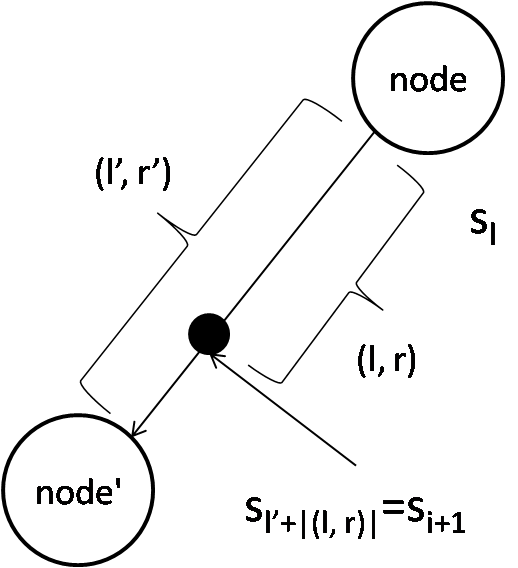
\includegraphics[scale=0.5]{img/implicit-end-point.eps}
  \caption{隐藏end point}
  \label{fig:implicit-end-point}
\end{figure}

Ukkonen发现了一个重要的事实:若$(node, (l, i))$是后缀树$SuffixTree(S_i)$的end point,则$(node, (l, i+1))$一定是后缀树$SuffixTree(S_{i+1})$的active point。

这是因为,如果$(node, (l, i))$是后缀树$SuffixTree(S_i)$的end point,它必然含有一个$s_{i+1}$子节点(可见的或者隐藏的)。如果end point代表后缀$s_ks_{k+1}...s_i$,它一定是后缀树$SuffixTree(S_i)$中最长的一个同时满足$s_ks_{k+1}...s_is_{i+1}$是$S_i$的某个子串的后缀。考虑$S_{i+1}$,由于后缀$s_ks_{k+1}...s_is_{i+1}$同时也是某个子串,它必然在$S_{i+1}$中至少出现两次,因此位置$(node, (l, i+1))$为后缀树$SuffixTree(S_{i+1})$的active point。图\ref{fig:ep-ap}给出了对应的解释。

\begin{figure}[htbp]
  \centering
  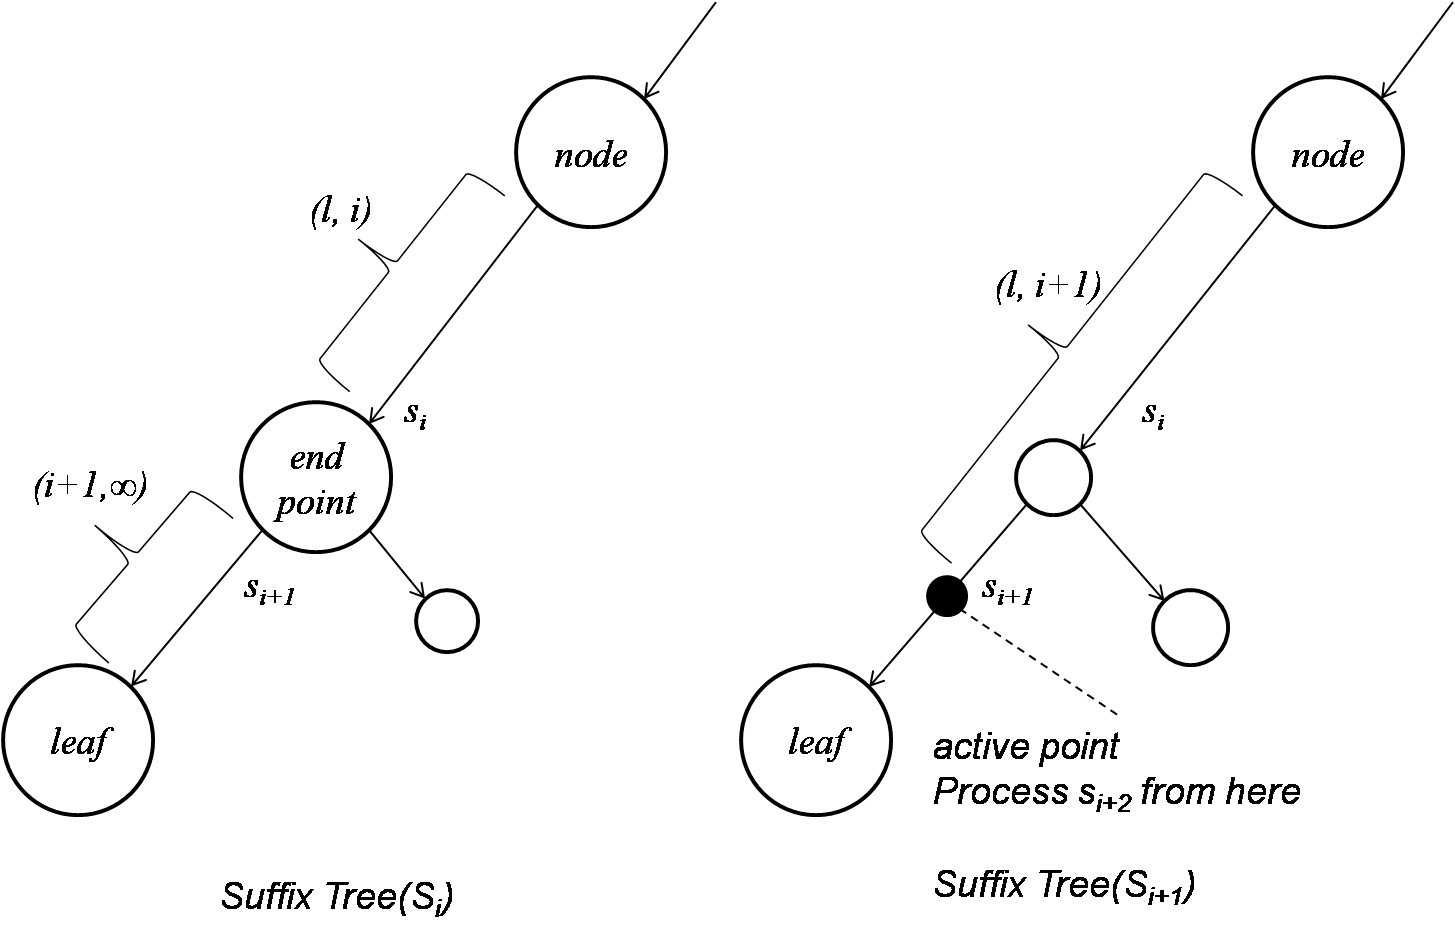
\includegraphics[scale=0.5]{img/ep-ap.eps}
  \caption{后缀树$SuffixTree(S_i)$的end point和后缀树$SuffixTree(S_{i+1})$的active point}
  \label{fig:ep-ap}
\end{figure}

总结以上各点,Ukkonen的on-line构造算法可以定义如下:

%\begin{algorithm}
\begin{algorithmic}[1]
\Function{Update}{$node, (l, i)$}
  \State $prev \gets$ \Call{Create-Empty-Node}{} \Comment{Initialized as sentinel} %
  \Loop \Comment{Traverse along the suffix links}
    \State $(finish, node') \gets$ \Call{End-Point-Branch?}{$node, (l, i-1), s_i$}
    \If{$finish$}
      \State break
    \EndIf
    \State \Call{Children}{$node'$}[$s_i$] $\gets$ ($(i, \infty)$, \Call{Create-Empty-Node}{})
    \State \Call{Suffix-Link}{$prev$} $\gets node'$
    \State $prev \gets node'$
    \State $(node, l) = $ \textproc{Canonize}(\Call{Suffix-Link}{$node$}, $(l, i-1)$)
  \EndLoop
  \State \Call{Suffix-Link}{$prev$} $\gets node$
  \State \Return $(node, l)$ \Comment{The end point}
\EndFunction
\end{algorithmic}
%\caption{Update $SuffixTree(S_{i-1})$}
%\label{algo:update}
%\end{algorithm}

算法接受一个引用对$(node, (l, i))$作为参数。这里$(node, (l, i-1)$是后缀树$SuffixTree(S_{i-1})$的active point。算法不断沿着后缀连接处理节点,直到位置$(node, (l, i-1))$成为end point。否则,函数\textproc{End-Point-Branch?}返回一个用于分支出新的叶子节点的位置。这个的实现如下:

%\begin{algorithm}
\begin{algorithmic}
\Function{End-Point-Branch?}{$node, (l, r), c$}
  \If{$(l, r) = \epsilon$}
    \If{$node = $ NIL}
      \State \Return (TRUE, $root$)
    \Else
      \State \Return (\Call{Children}{$node$}[$c$] = NIL, $node$)
    \EndIf
  \Else
    \State $((l', r'), node') \gets$ \Call{Children}{$node$}[$s_l$]
    \State $pos \gets l' + |(l, r)|$
    \If{$s_{pos} = c$}
      \State \Return (TRUE, $node$)
    \Else
      \State $p \gets$ \Call{Create-Empty-Node}{}
      \State \Call{Children}{$node$}[$s_{l'}$] $\gets ((l', pos-1), p)$
      \State \Call{Children}{$p$}[$s_{pos}$] $\gets ((pos, r'), node')$
      \State \Return (FALSE, $p$)
    \EndIf
  \EndIf
\EndFunction
\end{algorithmic}
%\caption{Test if a position is end point and create explicit node for further branching.}
%\label{algo:branch}
%\end{algorithm}

如果传入的位置是$(root, \epsilon)$,说明我们到达了根节点。根节点一定是end point,本轮的处理即可结束。如果传入的位置形如$(node, \epsilon)$,此引用对代表一个可见节点,我们可以检查它是否已经含有一个$c=s_i$的子节点。如果不含有,我们需要分支出一个新的叶子节点。

如果传入的不是一个可见节点的位置,也就是说$(node, (l, r))$指向一个隐藏节点。我们需要找到它的下一个位置以判断是否含有一个$c$子节点。如果含有,说明这是一个end point,我们可以结束本轮更新;否则,我们将此位置转化为一个可见节点,用于接下来分支出新的子节点。

Ukkonen算法最后实现如下:

%\begin{algorithm}
\begin{algorithmic}[1]
\Function{Suffix-Tree}{$S$}
  \State $root \gets$ \Call{Create-Empty-Node}{}
  \State $node \gets root, l \gets 0$
  \For{$i \gets 1$ to $|S|$}
    \State $(node, l) = $ \Call{Update}{$node, (l, i)$}
    \State $(node, l) = $ \Call{Canonize}{$node, (l, i)$}
  \EndFor
  \State \Return $root$
\EndFunction
\end{algorithmic}
%\caption{Main algorithm of Ukkonen's on-line construction for suffix tree.}
%\label{algo:ukkonen2}
%\end{algorithm}

图\ref{fig:cons-stree-cacao}给出了构造字符串“cacao”的后缀树的各个步骤。

\begin{figure}[htbp]
  \centering
  \subfloat[空]{\hspace{.1\textwidth}\includegraphics[scale=0.5]{img/strie-empty.ps}\hspace{.1\textwidth}}
  \subfloat[“c”]{\hspace{.1\textwidth}\includegraphics[scale=0.5]{img/stree-c.ps}\hspace{.1\textwidth}}
  \subfloat[“ca”]{\hspace{.1\textwidth}\includegraphics[scale=0.5]{img/stree-ca.ps}\hspace{.1\textwidth}} \\
  \subfloat[“cac”]{\hspace{.1\textwidth}\includegraphics[scale=0.5]{img/stree-cac.ps}\hspace{.1\textwidth}}
  \subfloat[“caca”]{\hspace{.1\textwidth}\includegraphics[scale=0.5]{img/stree-caca.ps}\hspace{.1\textwidth}}
  \subfloat[“cacao”]{\hspace{.1\textwidth}\includegraphics[scale=0.5]{img/stree-cacao.ps}\hspace{.1\textwidth}}
  \caption{构造字符串“cacao”的后缀树。公有6步。虚线箭头显示了最后一层的后缀连接。}
  \label{fig:cons-stree-cacao}
\end{figure}

我们并不需要为叶子节点设置后缀连接,只有分支节点需要后缀连接。

下面的Python例子程序实现了Ukkonen算法。首先是节点的定义:

\lstset{language=Python}
\begin{lstlisting}
class Node:
    def __init__(self, suffix=None):
        self.children = {} # 'c':(word, Node), where word = (l, r)
        self.suffix = suffix
\end{lstlisting}

为了节省空间,程序仅仅保留了一份完整的字符串,所有的子串都由左右边界对$(left, right)$来表示。对于叶子节点,右侧边界是开放的,用$(left, \infty)$来表示。后缀树的定义为:

\begin{lstlisting}
class STree:
    def __init__(self, s):
        self.str = s
        self.infinity = len(s)+1000
        self.root = Node()
\end{lstlisting}

在实际的程序中,使用完整字符串的长度加一来表示无穷。下面是一些辅助函数:

\begin{lstlisting}
def substr(str, str_ref):
    (l, r)=str_ref
    return str[l:r+1]

def length(str_ref):
    (l, r)=str_ref
    return r-l+1
\end{lstlisting}

Ukkonen算法的主函数实现如下:

\begin{lstlisting}
def suffix_tree(str):
    t = STree(str)
    node = t.root # init active point is (root, Empty)
    l = 0
    for i in range(len(str)):
        (node, l) = update(t, node, (l, i))
        (node, l) = canonize(t, node, (l, i))
    return t

def update(t, node, str_ref):
    (l, i) = str_ref
    c = t.str[i] # current char
    prev = Node() # dummy init
    while True:
        (finish, p) = branch(t, node, (l, i-1), c)
        if finish:
            break
        p.children[c]=((i, t.infinity), Node())
        prev.suffix = p
        prev = p
        (node, l) = canonize(t, node.suffix, (l, i-1))
    prev.suffix = node
    return (node, l)

def branch(t, node, str_ref, c):
    (l, r) = str_ref
    if length(str_ref)<=0: # (node, empty)
        if node is None: #_|_
            return (True, t.root)
        else:
            return ((c in node.children), node)
    else:
        ((l1, r1), node1) = node.children[t.str[l]]
        pos = l1+length(str_ref)
        if t.str[pos]==c:
            return (True, node)
        else:
            branch_node = Node()
            node.children[t.str[l1]]=((l1, pos-1), branch_node)
            branch_node.children[t.str[pos]] = ((pos, r1), node1)
            return (False, branch_node)

def canonize(t, node, str_ref):
    (l, r) = str_ref
    if node is None:
        if length(str_ref)<=0:
            return (None, l)
        else:
            return canonize(t, t.root, (l+1, r))
    while l<=r: # str_ref is not empty
        ((l1, r1), child) = node.children[t.str[l]]
        if r-l >= r1-l1:
            l += r1-l1+1
            node = child
        else:
            break
    return (node, l)
\end{lstlisting}

\subsubsection{函数式构造后缀树}
\index{后缀树!函数式构造}

Giegerich和Kurtz发现Ukkonen算法可以转化为McCreight算法\cite{GieKur97}。Weiner、McCreight和Ukkonen分别发现的三种后缀树构造算法都是线性时间复杂度$O(n)$的。Giegerich和Kurtz进一步猜想,任何后缀树的顺序构造算法如果不使用后缀链结或active后缀等概念,都无法达到线性时间复杂度的要求。

有一些Ukkonen算法的PLT/Scheme实现\cite{plt-stree},在处理中不断更新后缀链结。这样的实现不是纯函数式的。

现有的纯函数式实现通常依赖惰性编程环境,如Bryan O'Sullivan使用\cite{GieKur95}中的算法给出的Haskell实现\cite{Hackage-STree}。后缀树直到被查询或者遍历时才被按照需要构建。但是在不支持惰性求值的环境中,这一算法不能保证$O(n)$的性能。

下面的Haskell例子程序给出了后缀树的定义。一棵后缀树或是一个叶子;或者是一棵包含多棵子树的分支。每棵子树都对应一个字符串。

\lstset{language=Haskell}
\begin{lstlisting}
data Tr = Lf | Br [(String, Tr)] deriving (Eq)
type EdgeFunc = [String]->(String, [String])
\end{lstlisting}

函数edge从一组字符串列表中提取出公共前缀。注意这里并不要求edge函数一定要返回最长的公共前缀,它也可以返回一个空串(空串显然是任何字符串的前缀)。我们可以使用不同的edge函数来产生出不同的树。

\[
build(edge, X)
\]

这是一个通用的radix树构造函数。它使用一个edge函数从一组字符串中构造树。如果$X$是某个字符串的全部后缀,构造结果就是后缀trie或者后缀树。如果$X$是某个字符串的全部前缀,结果将会是前缀trie或者Patricia。

设所有字符串含有的字符集为$\Sigma$。若用于构造树的字符串为空,$X$仅仅包含一个空串,构造的结果为一个空的叶子节点;否则,我们检查$\Sigma$中的每个字符,将$X$中的字符串按照起始字符分组,然后在每一组上应用edge函数。

\be
build(edge, X) = \left \{
  \begin{array}
  {r@{\quad:\quad}l}
  leaf & X = \{ \phi \} \\
  \begin{array}{ll}
    branch(\{(\{c\} \cup p, & build(edge, X')) | \\
                            & c \in \Sigma, \\
                            & G \in \{ group(X, c) \}, \\
                            & (p, X') \in \{ edge(G) \} \})
  \end{array} & otherwise
  \end{array}
\right.
\ee

算法首先将全部的后缀按照首字符分成若干组,然后将每组中的首字符移除。例如,后缀$\{$“acac”, “cac”, “ac”, “c”$\}$被分成两组:$\{$(‘a’, [“cac”, “c”]), (‘c’, [“ac”, “”])$\}$。

\be
group(X, c) = \{C' | \{c_1\} \cup C' \in X, c_1 = c\}
\ee

函数$group$枚举$X$中的全部后缀,每个后缀的首字符记为$c_1$,余下字符记为$C'$。如果$c_1$和传入的字符$c$相等,则相应的$C'$就被归并到一组。

下面的Haskell例子程序实现了通用的radix树构造算法:

\begin{lstlisting}
alpha = ['a'..'z']++['A'..'Z']

lazyTree::EdgeFunc -> [String] -> Tr
lazyTree edge = build where
    build [[]] = Lf
    build ss = Br [(a:prefix, build ss') |
                         a<-alpha,
                         xs@(x:_) <-[[cs | c:cs<-ss, c==a]],
                         (prefix, ss')<-[edge xs]]
\end{lstlisting}

我们前面提到,不同的edge函数会导致构造出不同的radix树。唯一的要求就是edge函数能够提取出一组字符串的公共前缀。最简单的edge函数对任何输入都返回空串作为结果。这时我们会得到一棵trie。

\be
edgeTrie(X) = (\phi, X)
\ee

我们也可以实现一个edge函数,它能够提取出最长的公共前缀。这样的edge函数会构造出Patricia。记字符串列表为$X = \{x_1, x_2, ..., x_n\}$,对每个字符串$x_i$,令首字符为$c_i$,剩余的字符为$W_i$。若$X$仅含有一个字符串,最长的公共前缀显然就是这个字符串本身;如果$X$含有首字符不同的字符串,则公共前缀为空串;否则,所有的字符串的首字符都相同,这一首字符一定属于最长公共前缀。我们可以将所有字符串的首字符去除,然后递归地调用edge函数来寻找最长公共前缀。

\be
edgeTree(X) = \left \{
  \begin{array}
  {r@{\quad:\quad}l}
  (x_1, \{ \phi \}) & X = \{ x_1 \} \\
  (\phi, X) & |X| > 1, \exists x_i \in X, c_i \neq c_1 \\
  (\{c_1\} \cup p, Y) & (p, Y) = edgeTree(\{ W_i | x_i \in X \})
  \end{array}
\right.
\ee

下面列出函数$edgeTree$的一些例子。

\[
\begin{array}{l}
edgeTree(\{ \text{``an'', ``another'', ``and''}\}) = (\text{``an''}, \{\text{``'', ``other'', ``d''}\}) \\
edgeTree(\{ \text{``bool'', ``foo, ``bar''}\}) = (\text{``''}, \{\text{``bool'', ``fool'', ``bar''}\})
\end{array}
\]

下面的Haskell例子程序实现了提取最长公共前缀的edge函数。

\begin{lstlisting}
edgeTree::EdgeFunc
edgeTree [s] = (s, [[]])
edgeTree awss@((a:w):ss) | null [c|c:_<-ss, a/=c] = (a:prefix, ss')
                         | otherwise              = ("", awss)
                         where (prefix, ss') = edgeTree (w:[u| _:u<-ss])
edgeTree ss = ("", ss)
\end{lstlisting}

给定任意字符串,我们可以通过使用上面的两个edge函数来构造后缀trie和后缀树。

\be
suffixTrie(S) = build(edgeTrie, suffixes(S))
\ee

\be
suffixTree(S) = build(edgeTree, suffixes(S))
\ee

由于$build(edge, X)$的通用性,它也可以用于构造普通的前缀trie和Patricia等radix树:

\be
trie(S) = build(edgeTrie, prefixes(S))
\ee

\be
tree(S) = build(edgeTree, prefixes(S))
\ee

% ================================================================
%               Suffix tree applications
% ================================================================

\section{后缀树的应用}

后缀树可以高效地处理很多字符串操作和DNA匹配相关的问题。

\subsection{字符串搜索和模式匹配}
\label{substring-lookup}
\index{后缀树!字符串搜索}

字符串搜索的算法非常丰富,例如著名的KMP(Knuth-Morris-Pratt)算法,本书搜索一章专门介绍了这一算法。后缀树的搜索效率和KMP算法相当\cite{zhang-shaojie-lec}。如果待搜索的子串长度为$m$,后缀树的搜索时间为$O(m)$。但是我们需要$O(n)$的时间来预先构造搜索树,其中$n$是搜索文本的长度\cite{lallison-stree}。

不仅是字符串搜索,后缀树还可以用来实现模式匹配甚至包括正则表达式。Ukkonen将这类问题称为子串motif。他指出:“即使字符串$S$可能含有$O(n^2)$个子串。$SuffixTree(S)$也可以在$O(n)$时间内找出任何子串motif的出现次数。”

\subsubsection{子串出现的次数}
\index{后缀树!子串出现的次数}

$SuffixTree(S)$中,任意内部节点都代表一个在字符串$S$中出现一次以上的子串。如果子串在$S$中出现$k$次,则其对应的节点含有$k$个子分支\cite{ukkonen-lec}。

\begin{algorithmic}[1]
\Function{Lookup-Pattern}{$T, s$}
  \Loop
    \State $match \gets$ FALSE
    \For{$\forall (s_i, T_i) \in$ \textproc{Values}(\Call{Children}{$T$})}
      \If{$s \sqsubset s_i$}
        \State \Return \textproc{Max}($|$\Call{Children}{$T_i$}$|$, 1)
      \ElsIf{$s_i \sqsubset s$}
        \State $match \gets$ TRUE
        \State $T \gets T_i$
        \State $s \gets s - s_i$
        \State break
      \EndIf
    \EndFor
    \If{$\lnot match$}
      \State \Return 0
    \EndIf
  \EndLoop
\EndFunction
\end{algorithmic}

当从文本$w$中寻找子串$s$时,我们首先从$w$构造后缀树$T$。从根节点开始,我们遍历所有子节点。针对每个子串$s_i$和子树$T_i$对,检查$s$是否是$s_i$的前缀。如果是,就返回$T_i$的子分支个数作为结果。有一种特殊情况:$T_i$是一个叶子节点,而没有任何子节点。这种情况下我们需要返回1,而不是0。因此上述实现中,我们使用了max函数。反之,如果$s_i$是$s$的前缀,我们就从$s$中去掉$s_i$这一部分,然后递归地在$T_i$中查找。

下面的Python例子程序实现了这一算法。

\lstset{language=Python}
\begin{lstlisting}
def lookup_pattern(t, s):
    node = t.root
    while True:
        match = False
        for _, (str_ref, tr) in node.children.items():
            edge = substr(t, str_ref)
            if string.find(edge, s)==0: #s `isPrefixOf` edge
                return max(len(tr.children), 1)
            elif string.find(s, edge)==0: #edge `isPrefixOf` s
                match = True
                node = tr
                s = s[len(edge):]
                break
        if not match:
            return 0
    return 0 # not found
\end{lstlisting}

也可以用递归的方式查找子串出现的次数。若后缀树$T$不是一个简单的叶子节点,记$C$为$T$之下的全部子串—子树映射对$C = \{(s_1, T_1), (s_2, T_2), ...\}$。我们在这组子树中查找子串。

\be
lookup_{pattern}(T, s) = find(C, s)
\ee

如果$C$为空,说明子串没有出现过;否则,我们检查第一对映射$(s_1, T_1)$,如果$s$是$s_1$的前缀,则子树$T_1$的子分支数目就是结果。如果$s_1$是$s$的子串,我们从$s$中去除$s_1$的部分,然后递归在$T_1$中查找;否则,我们继续在剩余的子串—子树映射$C'$中进行同样的处理。

\be
find(C, s) = \left \{
  \begin{array}
  {r@{\quad:\quad}l}
  0 & C = \phi \\
  max(1, |C_1|) & s \sqsubset s_1 \\
  lookup_{pattern}(T_1, s - s_1) & s_1 \sqsubset s \\
  find(C', s) & otherwise
  \end{array}
\right.
\ee

下面的Haskell例子程序实现了这一算法。

\lstset{language=Haskell}
\begin{lstlisting}
lookupPattern (Br lst) ptn = find lst where
    find [] = 0
    find ((s, t):xs)
         | ptn `isPrefixOf` s = numberOfBranch t
         | s `isPrefixOf` ptn = lookupPattern t (drop (length s) ptn)
         | otherwise = find xs
    numberOfBranch (Br ys) = length ys
    numberOfBranch _ = 1

findPattern s ptn = lookupPattern (suffixTree $ s++"$") ptn
\end{lstlisting}

我们总是在字符串末尾增加一个特殊的终结符(上述程序中使用‘\$’作为终结符),这样就可以避免某个后缀也同时成为其它后缀的前缀\cite{wiki-suffix-tree}。

后缀树也可以用来搜索“a**n”这样的模式,本书略过了这些内容,读者可以参考\cite{ukkonen-lec}或\cite{ukkonen-search}来了解其中的细节。

\subsection{查找最长重复子串}
\index{最长重复子串}
\underline{向字符串S增加一个特殊的终结符,我们可以通过在后缀树中搜索最深分支来找到最长重复子串。}

考虑图\ref{fig:stree-mississippis}中的后缀树。

\begin{figure}[htbp]
  \centering
  \includegraphics[scale=0.5]{img/stree-mississippis.ps}
  \caption{字符串‘mississippi\$’对应的后缀树。} \label{fig:stree-mississippis}
\end{figure}

深度为3的分支节点有3个,分别是$A$、$B$和$C$。其中$A$代表了最长重复子串“issi”,$B$代表“si”,$C$代表“ssi”,它们都比$A$代表的子串短。

这个例子说明,分支的“深度”应该用从根节点开始到达分支所经过的字符数目来衡量,而不是使用可见分支节点的个数来衡量。

下面的广度优先搜索算法,可以在后缀树中找到最长重复子串。

\begin{algorithmic}[1]
\Function{Longest-Repeated-Substring}{$T$}
  \State $Q \gets$ (NIL, \Call{Root}{$T$})
  \State $R \gets$ NIL
  \While{$Q$ is not empty}
    \State $(s, T) \gets$ \Call{Pop}{$Q$}
    \For{each $((l, r), T') \in$ \Call{Children}{$T$}}
      \If{$T'$ is not leaf}
        \State $s' \gets$ \Call{Concatenate}{$s, (l, r)$}
        \State \Call{Push}{$Q, (s', T')$}
        \State $R \gets$ \Call{Update}{$R, s'$}
      \EndIf
    \EndFor
  \EndWhile
  \State \Return $R$
\EndFunction
\end{algorithmic}

算法使用一个队列来进行搜索,队列一开始含有一对元素,包括一个空串和根节点。然后算法不断从队列中取出候选元素进行处理。

针对每个节点,算法都逐一检查它的所有子树。如果是一个分支节点,这个子树就被放回队列等待后继的搜索。它对应的子串就被作为最长重复子串的候选。

函数\textproc{Update}($R, s'$)用于更新候选的最长重复子串。如果存在多个长度相同的子串,它们就被放入一个结果列表。

\begin{algorithmic}[1]
\Function{Update}{$L, s$}
  \If{$L =$ NIL $\lor |l_1| < |s|$}
    \State \Return $l \gets \{ s \}$
  \EndIf
  \If {$|l_1| = |s|$}
    \State \Return \Call{Append}{$L, s$}
  \EndIf
  \State \Return $L$
\EndFunction
\end{algorithmic}

下面的Python例子程序实现了这一算法。

\lstset{language=Python}
\begin{lstlisting}
def lrs(t):
    queue = [("", t.root)]
    res = []
    while len(queue)>0:
        (s, node) = queue.pop(0)
        for _, (str_ref, tr) in node.children.items():
            if len(tr.children)>0:
                s1 = s+t.substr(str_ref)
                queue.append((s1, tr))
                res = update_max(res, s1)
    return res

def update_max(lst, x):
    if lst ==[] or len(lst[0]) < len(x):
        return [x]
    if len(lst[0]) == len(x):
        return lst + [x]
    return lst
\end{lstlisting}

我们也可以用递归的方式搜索最长重复子串。如果待搜索的树是一个叶子节点,结果为空串;否则算法在子树中寻找最长重复子串。

\be
LRS(T) = \left \{
  \begin{array}
  {r@{\quad:\quad}l}
  \phi & leaf(T) \\
  longest(\{s_i \cup LRS(T_i) | (s_i, T_i) \in C, \lnot leaf(T_i)\}) & otherwise
  \end{array}
\right.
\ee

下面的Haskell例子程序实现了最长重复子串的算法。

\lstset{language=Haskell}
\begin{lstlisting}
isLeaf Lf = True
isLeaf _ = False

lrs' Lf = ""
lrs' (Br lst) = find $ filter (not . isLeaf . snd) lst where
    find [] = ""
    find ((s, t):xs) = maximumBy (compare `on` length) [s++(lrs' t), find xs]
\end{lstlisting} %$

\subsection{查找最长公共子串}
\index{最长公共子串}

后缀树还可以用来查找多个字符串的最长公共字串。我们先考虑两个字符串的情况。记这两个串为$txt_1$和$txt_2$,我们可以构造一棵后缀树$SuffixTree(txt_1\$_1txt_2\$_2)$。其中$\$_1$是$txt_1$的特殊终结符;$\$_2 \neq \$_1$是$txt_2$的特殊终结符。

为了获得最长公共字串,我们只需要找到最深的一个分支节点,它同时包含形如“...$\$_1$...”和“...$\$_2$”(不含$\$_1$)的两个叶子。这里“最深”节点的含意和前面最长重复字串中的一致:深度为从根节点算起的字符个数。

如果一个节点含有代表“...$\$_1$...”的叶子,这个节点一定对应$txt_1$的某个子串。同时,由于它也含有一个代表“...$\$_2$”(不含$\$_1$)的叶子,这个节点一定也对应到$txt_2$的某个子串。如果它是所有这类节点中最深的一个,它一定对应着最长的公共子串。

我们可以使用类似的广度优先(BFS)算法来查找最长公共子串。

\begin{algorithmic}[1]
\Function{Longest-Common-Substring}{$T$}
  \State $Q \gets$ (NIL, \Call{Root}{$T$})
  \State $R \gets$ NIL
  \While{$Q$ is not empty}
    \State $(s, T) \gets$ \Call{POP}{$Q$}
    \If{\Call{Match-Fork}{$T$}}
      \State $R \gets$ \Call{Update}{$R, s$}
    \EndIf
    \For{each $((l, r), T') \in $ \Call{Children}{$T$}}
      \If{$T'$ is not leaf}
        \State $s' \gets$ \Call{Concatenate}{$s, (l, r)$}
        \State \Call{Push}{$Q, (s', T')$}
      \EndIf
    \EndFor
  \EndWhile
  \State \Return $R$
\EndFunction
\end{algorithmic}

大部份实现和最长重复子串的查找算法相同。函数\textproc{Match-Fork}用以检查一个节点是否含有两个满足公共子串的叶子节点。

\begin{algorithmic}[1]
\Function{Match-Fork}{$T$}
  \If{$|$ \Call{Children}{$T$} $| = 2$}
    \State $\{(s_1, T_1), (s_2, T_2)\} \gets$ \Call{Children}{$T$}
    \State \Return $T_1$ is leaf $\land T_2$ is leaf $\land$ \Call{Xor}{$\$_1 \in s_1, \$_1 \in s_2)$}
  \EndIf
  \State \Return FALSE
\EndFunction
\end{algorithmic}

这个函数检查一个节点是否含有两个叶子节点,其中一个含有$\$_2$,而另外一个不含有。这是因为如果一个节点是叶子节点,根据后缀树的定义,它一定包含终结符$\$_1$。

下面的Python例子程序实现了最长公共子串的查找算法。

\lstset{language=Python}
\begin{lstlisting}
def lcs(t):
    queue = [("", t.root)]
    res = []
    while len(queue)>0:
        (s, node) = queue.pop(0)
        if match_fork(t, node):
            res = update_max(res, s)
        for _, (str_ref, tr) in node.children.items():
            if len(tr.children)>0:
                s1 = s + t.substr(str_ref)
                queue.append((s1, tr))
    return res

def is_leaf(node):
    return node.children=={}

def match_fork(t, node):
    if len(node.children)==2:
        [(_, (str_ref1, tr1)), (_, (str_ref2, tr2))]=node.children.items()
        return is_leaf(tr1) and is_leaf(tr2) and
            (t.substr(str_ref1).find('#')!=-1) !=
            (t.substr(str_ref2).find('#')!=-1)
    return False
\end{lstlisting}

The longest common sub-string finding algorithm can also be
realized recursively. If the suffix tree $T$ is a leaf, the result is empty;
Otherwise, we examine all children in $T$. For those satisfy the matching
criteria, the sub-string are collected as candidates; for those don't
matching, we recursively search the common sub-string among the children.
The longest candidate is selected as the final result.

\be
LCS(T) = \left \{
  \begin{array}
  {r@{\quad:\quad}l}
  \phi & leaf(T) \\
  \begin{array}{ll}
    longest( & \{s_i | (s_i, T_i) \in C, match(T_i)\} \cup \\
             & \{s_i \cup LCS(T_i) | (s_i, T_i) \in C, \lnot match(T_i)\})
  \end{array} & otherwise
  \end{array}
\right.
\ee

The following Haskell example program implements the longest common sub-string algorithm.

\lstset{language=Haskell}
\begin{lstlisting}
lcs Lf = []
lcs (Br lst) = find $ filter (not .isLeaf . snd) lst where
    find [] = []
    find ((s, t):xs) = maxBy (compare `on` length)
                       (if match t
                        then s:(find xs)
                        else  (map (s++) (lcs t)) ++ (find xs))

match (Br [(s1, Lf), (s2, Lf)]) = ("#" `isInfixOf` s1) /= ("#" `isInfixOf` s2)
match _ = False
\end{lstlisting}

\subsection{Find the longest palindrome}
\index{Longest palindrome}

A palindrome is a string, $S$, such that $S=reverse(S)$ For example,
``level'', ``rotator'', ``civic'' are all palindrome.

The longest palindrome in a string $s_1s_2...s_n$ can be found in
$O(n)$ time with suffix tree. The solution can be benefit from the
longest common sub-string algorithm.

For string $S$, if sub-string $w$ is a palindrome, then it must be
sub-string of $reverse(S)$ too. for instance, ``issi'' is a palindrome,
it is a sub-string of ``mississippi''. When reverse to
``ippississim'', ``issi'' is also a sub-string.

Based on this fact, we can find the longest palindrome by
searching the longest common sub-string for $S$ and $reverse(S)$.

\be
palindrome_m(S) = LCS(suffixTree(S \cup reverse(S)))
\ee

The following Haskell example program finds the longest palindrome.

\lstset{language=Haskell}
\begin{lstlisting}
longestPalindromes s = lcs $ suffixTree (s++"#"++(reverse s)++"$")
\end{lstlisting}

\subsection{Others}
Suffix tree can also be used for data compression, such as Burrows-Wheeler
transform, LZW compression (LZSS) etc. \cite{wiki-suffix-tree}

% ================================================================
%                 Short summary
% ================================================================
\section{Notes and short summary}

Suffix Tree was first introduced by Weiner in 1973 \cite{weiner}.
In 1976, McCreight greatly simplified the construction algorithm.
McCreight constructs the suffix tree from right to left. In 1995,
Ukkonen gave the first on-line construction algorithms from
left to right. All the three algorithms are linear time ($O(n)$).
And some research shows the relationship among these 3 algorithms.
\cite{GieKur97}

\begin{thebibliography}{99}

\bibitem{ukkonen95}
Esko Ukkonen. ``On-line construction of suffix trees''. Algorithmica 14 (3): 249--260. doi:10.1007/BF01206331. http://www.cs.helsinki.fi/u/ukkonen/SuffixT1withFigs.pdf

\bibitem{weiner73}
Weiner, P. ``Linear pattern matching algorithms'', 14th Annual IEEE Symposium on Switching and Automata Theory, pp. 1-11, doi:10.1109/SWAT.1973.13

\bibitem{wiki-suffix-tree}
Suffix Tree, Wikipedia. http://en.wikipedia.org/wiki/Suffix\_tree

\bibitem{ukkonen-presentation}
Esko Ukkonen. ``Suffix tree and suffix array techniques for pattern analysis in strings''. http://www.cs.helsinki.fi/u/ukkonen/Erice2005.ppt

\bibitem{wiki-trie}
Trie, Wikipedia. http://en.wikipedia.org/wiki/Trie

\bibitem{trivial-stree-java}
Suffix Tree (Java). http://en.literateprograms.org/Suffix\_tree\_(Java)

\bibitem{GieKur97}
Robert Giegerich and Stefan Kurtz. ``From Ukkonen to McCreight and Weiner: A Unifying View of Linear-Time Suffix Tree Construction''. Science of Computer Programming 25(2-3):187-218, 1995. http://citeseer.ist.psu.edu/giegerich95comparison.html

\bibitem{GieKur95}
Robert Giegerich and Stefan Kurtz. ``A Comparison of Imperative and Purely Functional Suffix Tree Constructions''. Algorithmica 19 (3): 331--353. doi:10.1007/PL00009177. www.zbh.uni-hamburg.de/pubs/pdf/GieKur1997.pdf

\bibitem{Hackage-STree}
Bryan O'Sullivan. ``suffixtree: Efficient, lazy suffix tree implementation''. http://hackage.haskell.org/package/suffixtree

\bibitem{plt-stree}
Danny. http://hkn.eecs.berkeley.edu/~dyoo/plt/suffixtree/

\bibitem{zhang-shaojie-lec}
Zhang Shaojie. ``Lecture of Suffix Trees''. http://www.cs.ucf.edu/~shzhang/Combio09/lec3.pdf

\bibitem{lallison-stree}
Lloyd Allison. ``Suffix Trees''. http://www.allisons.org/ll/AlgDS/Tree/Suffix/

\bibitem{ukkonen-lec}
Esko Ukkonen. ``Suffix tree and suffix array techniques for pattern analysis in strings''. http://www.cs.helsinki.fi/u/ukkonen/Erice2005.ppt

\bibitem{ukkonen-search}
Esko Ukkonen ``Approximate string-matching over suffix trees''. Proc. CPM 93. Lecture Notes in Computer Science 684, pp. 228-242, Springer 1993. http://www.cs.helsinki.fi/u/ukkonen/cpm931.ps

\end{thebibliography}

\ifx\wholebook\relax \else
\end{document}
\fi
